%%% PREAMBLE

\documentclass[11pt]{report}
\usepackage[utf8]{inputenc}
% This is in order to have the chapter feature
% and page numbers in the same location on even and odd pages.
% Acceptable font sizes are 10 to 12 pts

%%% Header for dissertation
%%% Caleb Stanford
%%% Summer 2022

% Official template:
% https://github.com/danieldeutsch/upenn-cis-templates/blob/master/thesis/thesis.tex

%% ========== Official Preamble ==========
% (with some minor modifications)

\usepackage[papersize={8.5 in, 11 in}, nohead, includeheadfoot, left=1.5 in, right = 1 in, vmargin= 1 in]{geometry}
% The options above are to set the paper size (as per page 11 of the guidelines and the margins. Includefoot is to make sure that nothing
% gets printed on the margins. The statutory margins are set on page 5.

\usepackage[doublespacing]{setspace} % Needed to set double-spacing for the main document, but needs more adhoc commands to
								% use single spacing for tables, etc.
\usepackage{calc}
% https://tex.stackexchange.com/questions/212710/fill-space-created-by-phantom-with-other-text
\newcommand{\textover}[3][l]{%
 % #1 is the alignment, default l
 % #2 is the text to be printed
 % #3 is the text for setting the width
 \makebox[\widthof{#3}][#1]{#2}%
}

\usepackage{microtype}

% For the signature boxes and much better looking tables
\usepackage{array} % Also for better arrays (eg matrices) in maths
\usepackage{tabularx}
\usepackage{booktabs}
\usepackage{makecell} % Line breaks in tables

% Commands to format the Table of Contents, List of Tables and List of Illustrations, as per the Wharton Template
\usepackage{tocloft}
\setcounter{tocdepth}{2} % Only show chapters and sections in ToC

% Change names and format of tables
\renewcommand{\contentsname}{TABLE OF CONTENTS}
\renewcommand{\cfttoctitlefont}{\large\hfill}
\renewcommand{\cftaftertoctitle}{\hfill}
\renewcommand{\cftbeforetoctitleskip}{-21 pt} % The key value here is the -21 pts, I got to it by old fashioned measuring with a ruler....
\renewcommand{\listtablename}{LIST OF TABLES}
\renewcommand{\cftlottitlefont}{\large\hfill}
\renewcommand{\cftafterlottitle}{\hfill}
\renewcommand{\cftbeforelottitleskip}{-21 pt} % The key value here is the -21 pts, I got to it by old fashioned measuring with a ruler....
\renewcommand{\listfigurename}{LIST OF ILLUSTRATIONS}
\renewcommand{\cftloftitlefont}{\large\hfill}
\renewcommand{\cftafterloftitle}{\hfill}
\renewcommand{\cftbeforeloftitleskip}{-21 pt} % The key value here is the -21 pts, I got to it by old fashioned measuring with a ruler....

% Format chapters (dots, including the word chapter, etc.)
\renewcommand{\cftchapfont}{\upshape}
\renewcommand{\cftchapleader}{\upshape\cftdotfill{\cftdotsep}}
\renewcommand{\cftchappagefont}{\upshape}
\renewcommand{\cftchappresnum}{CHAPTER }
\renewcommand{\cftchapaftersnum}{ :}
\newlength{\mylen}   % a "scratch" length
\settowidth{\mylen}{\cftchappresnum \cftchapaftersnum} % extra space
\addtolength{\cftchapnumwidth}{\mylen} % add the extra space

%% Suppressing some annoying warnings
% "PDF inclusion: multiple pdfs with page group included in a single page"
% https://tex.stackexchange.com/a/78020/28267
\pdfsuppresswarningpagegroup=1
% "PDF inclusion: found PDF version <1.6>, but at most version <1.5> allowed"
% https://tex.stackexchange.com/questions/52317/pdftex-warning-version-allowed
\pdfminorversion=6
% "Package remreset Warning: The remreset package is obsolete"
% https://tex.stackexchange.com/questions/438543/what-to-do-when-an-actively-maintained-package-requires-an-obsolete-package
\RequirePackage{silence}
\WarningFilter{remreset}{The remreset package}

% Format tables in LoT
\renewcommand{\cfttableader}{\cftdotfill{\cftdotsep}}
\renewcommand{\cfttabpresnum}{TABLE }
\renewcommand{\cfttabaftersnum}{ :}
\newlength{\mylent}   % a "scratch" length
\settowidth{\mylent}{\cfttabpresnum} % extra space
\addtolength{\cfttabnumwidth}{\mylent} % add the extra space
\usepackage{remreset}

% Format Illusstrations in LoF
\renewcommand{\cftfigleader}{\cftdotfill{\cftdotsep}}
\renewcommand{\cftfigpresnum}{FIGURE }
\renewcommand{\cftfigaftersnum}{ :}
\newlength{\mylenf}   % a "scratch" length
\settowidth{\mylenf}{\cftfigpresnum} % extra space
\addtolength{\cftfignumwidth}{\mylenf} % add the extra space

% Commands (more further down, at preliminary, main and appendix) to change the formatting of chapter headings
\usepackage[compact]{titlesec}
\renewcommand{\beforetitleunit}{0 pt}
\titleformat{\section}[hang]{\large}{\thesection.}{6 pt}{}
\titleformat{\subsection}[hang]{\normalsize\itshape}{\thesubsection.}{6 pt}{}
\titlespacing*{\section}{0pt}{20pt}{8pt}
\titlespacing*{\subsection}{0pt}{10pt}{6pt}

\usepackage{parskip} % To allow for better management of the Dutch paragraph style
\usepackage{url} % To allow for better typing of the url in the Creative Commons part of the copyright
% TODO include this again?
% \usepackage{natbib} % allows the author-date citation system
% \bibpunct{(}{)}{;}{a}{,}{,} % options for natbib to yield the citation style I like

% Other packages that are not needed for the template, but I highly recommend (and all of your own packages go here to)
% Add them one by one to make sure they do not interfere, for instance the package subfigure clashes with this template
\usepackage{amssymb}
% \usepackage{amsfonts}
\usepackage{amsmath}
\usepackage{graphicx}
% \usepackage{longtable}
% \usepackage{dcolumn}
% \usepackage{longtable}
% \usepackage{rotating}
% \usepackage{xtab}               % collides on tablehead with glossaries
% \usepackage{paralist} % very flexible & customizable lists (eg. enumerate/itemize, etc.)
% \usepackage{verbatim}
% \usepackage{subfiles} % To be better able to manage large projects by compiling the separate files included in the final document

% FOR ADDING LINE NO. I have checked, this does not mess with margins (i.e. the # appears outside the margins, so no new orphans/widows are introduced)
% TODO: comment out for final version
\usepackage{lineno}
\linenumbers

%% TO TURN ON BIB FOR CHAPTER (when compiling chapters separately)
% \def\biblio{\bibliographystyle{abbrvnat}\bibliography{thesis}}
% %% TO TURN OFF BIB FOR EACH CHAPTER, (for compiling the whole thesis)
\def\biblio{}

%% ========== General ==========

% Theorems
\usepackage{amsthm}
\theoremstyle{definition}
\newtheorem{theorem}{Theorem}
\newtheorem{lemma}[theorem]{Lemma}
\newtheorem{proposition}[theorem]{Proposition}
\newtheorem{definition}[theorem]{Definition}
\newtheorem{example}[theorem]{Example}
\numberwithin{theorem}{section}

% Inference rules
\usepackage{mathpartir}
\newcommand{\inference}[3][]{\inferrule*[Right=#1]{#2}{#3}}

% Clickable links & references
\usepackage{hyperref}
% TODO: underline links
\hypersetup{
    colorlinks,
    linkcolor={red!50!black},
    citecolor={blue!50!black},
    urlcolor={blue!80!black}
}
% Abbreviation
\newcommand{\githubref}[2]{\href{#1}{#2}\footnote{\url{#1}}}

% Multiple bibliography -- primary references & other
\usepackage{cleveref}
\usepackage{multibib}
\newcites{Main}{PRIMARY REFERENCES}

%% ========== Document layout ==========

%% Roman Numerals
\makeatletter
\newcommand*{\romnum}[1]{\romannumeral #1\relax}
\newcommand*{\RomNum}[1]{\expandafter\@slowromancap\romannumeral #1@}
\makeatother

% Fancy custom section headers

\usepackage{changepage}
% \usepackage{titlesec}
% \titleformat{\section}[display]
%   {%
%     \clearpage\thispagestyle{empty}%
%     \normalfont\Large\bfseries\filcenter\titlerule[1pt]\vskip3pt%
%   }
%   {\RomNum{\thesection}.}
%   {-2pt}
%   {}
%   [{\vskip5pt\titlerule[1pt]\vspace{0.5cm}}]

\newcommand{\headerblock}[1]{
  \begin{adjustwidth}{1cm}{1cm}
  \begin{center}
    #1
  \end{center}
\end{adjustwidth}
  \vspace{0.5cm}
  % \clearpage
}
\newcommand{\headerimage}[1]{\includegraphics[width=0.7\textwidth]{#1}}
\newcommand{\headerquote}[2]{\textit{#1 \qquad} \\ \qquad ---#2}
\newcommand{\headerbreak}{\vspace{0.5cm}}
% Hide for official version
\newcommand{\headerhide}[1]{}

%% ========== Graphics and symbols ==========

\usepackage[dvipsnames]{xcolor}
\usepackage{graphbox} % allows using [align=c] argument to center vertically
\usepackage{stmaryrd} % Symbols like \llbracket, \rrbracket
\usepackage{pifont} % Symbols like \ding
\usepackage{relsize} % Large symbols (\mathlarger)

\newcommand{\GreenYes}{\color{ForestGreen}{Yes}}
\newcommand{\RedNo}{\color{red}{No}}
\newcommand{\cmark}{\ding{51}}
\newcommand{\xmark}{\ding{55}}

%% ========== TikZ ==========

\usepackage{tikz}
\usetikzlibrary{positioning, matrix, fit, arrows, shapes}
\usetikzlibrary{fit}

%% Block Diagrams
\tikzset{Block/.style={draw, rectangle, inner sep=4pt, align=center}}
\tikzset{Block Edge/.style={draw,thick,->}}
% \tikzset{Data/.append style={ellipse}}
% \tikzset{Input/.append style={fill=red!20}}
% \tikzset{Output/.append style={fill=blue!20}}
\tikzset{Data/.append style={fill=blue!20}}
\tikzset{Input/.append style={}}
\tikzset{Output/.append style={}}

%% Dataflow Graphs
\tikzset{source/.style={
        draw,
        rounded rectangle,
        inner sep=2pt,
        align=center,
        fill=blue!20
}}
\tikzset{operator/.style={
        draw,
        rectangle,
        inner sep=2pt,
        align=center
}}
\tikzset{sink/.style={
        draw,
        rounded rectangle,
        inner sep=2pt,
        align=center,
        fill=blue!20
}}
\tikzset{dataflowedge/.style={draw,thick,->}}

%% Topology Diagrams
\tikzset{Device Node/.style={draw,circle}}
\tikzset{Network/.style={draw,cloud,cloud puffs=10,cloud puff arc=120, aspect=2.5, inner sep=2pt}}
\tikzset{In Edge/.style={->,very thick,red}}
\tikzset{Out Edge/.style={->,very thick,blue}}

% Dependency Relations
\tikzset{Tag Node/.style={draw, circle, inner sep=0.5pt}}
\tikzset{Tag Edge/.style={draw, thick}}
\tikzset{Tag Loop/.style={draw, thick, in=245, out=305, looseness=5}}
\newcommand{\KeyDepGraph}[1]{
    \begin{tikzpicture}[baseline=(1.base)]
        \node[Tag Node] (1) at (0,0) {\tg{#1}$_1$};
        \draw (1) edge[Tag Loop] (1);
        \node[Tag Node] (2) at (1.2,0) {\tg{#1}$_2$};
        \node[draw=none,fill=none] at (2.1,0) {$\cdots$};
        \draw (2) edge[Tag Loop] (2);
        \node[Tag Node] (3) at (3,0) {\tg{#1}$_k$};
        \node[draw=none,fill=none] at (3.9,0) {$\cdots$};
        \draw (3) edge[Tag Loop] (3);
    \end{tikzpicture}}
\newcommand{\ExtendedKeyDepGraph}[1]{
    \begin{tikzpicture}[baseline=(1.base)]
        \node[Tag Node] (1) at (0,0) {\tg{#1}$_1$};
        \draw (1) edge[Tag Loop] (1);
        \node[Tag Node] (2) at (1.2,0) {\tg{#1}$_2$};
        \node[draw=none,fill=none] at (2.1,0) {$\cdots$};
        \draw (2) edge[Tag Loop] (2);
        \node[Tag Node] (3) at (3,0) {\tg{#1}$_k$};
        \node[draw=none,fill=none] at (3.9,0) {$\cdots$};
        \draw (3) edge[Tag Loop] (3);
        \node[Tag Node] (4) at (1.6,1.2) {\tg{EOD}};
        \draw (4) edge[Tag Loop, in=65, out=115] (4);
        \draw (1) edge[Tag Edge] (4);
        \draw (2) edge[Tag Edge] (4);
        \draw (3) edge[Tag Edge] (4);
        \node[Tag Node] (5) at (0,1.2) {\tg{EOM}};
        \draw (5) edge[Tag Loop, in=65, out=115] (5);
        \draw (4) edge[Tag Edge] (5);
    \end{tikzpicture}}

%% update/fork/join computations
\tikzset{B/.style={draw, inner sep=0pt, circle, font=\footnotesize{}, minimum size=16pt}}
% minimum size=16pt
% regular polygon, regular polygon sides=4,font=\footnotesize}}
\tikzset{E/.style={draw,->}}
\tikzset{W/.style={draw, font=\small}}

\newcommand{\TwoTagDepGraph}[3]{
    \begin{tikzpicture}[baseline=(1.base)]
        \node[Tag Node] (1) at (210:0.5) {\footnotesize #1};
        \node[Tag Node] (2) at (330:0.5) {\footnotesize #2};
        #3
    \end{tikzpicture}}
% \newcommand{\ThreeTagDepGraph}[4]{
%     \begin{tikzpicture}[baseline=(1.base)]
%         \node[Tag Node] (1) at (90:0.3) {#1};
%         \node[Tag Node] (2) at (210:0.5) {#2};
%         \node[Tag Node] (3) at (330:0.5) {#3};
%         #4
%     \end{tikzpicture}}
\newcommand{\TopConfigNode}[3]{
    \begin{tabular}{c | c }
        #1 & \{ #2 \} \\
        \hline
        \multicolumn{2}{c}{#3}
    \end{tabular}
}

\newcommand{\ConfigurationNode}[3]{
    node { \TopConfigNode{#1}{#2}{#3} } }

\newcommand{\TopWorkerNode}[3]{

%     \matrix (M) {
%         || #1 \\
%         Independent \\
%         Reduction \\
%         DivideAndConquer \\
%     };
%   \draw[black] (M-2-1.north west) -- (M-2-1.north east);

    \begin{tabular}{c}
        #1 \\
        \hline
        \{ #2 \} \\
        {#3}
    \end{tabular}
}
\newcommand{\TopDNode}[4]{
    % \begin{tabular}{c c c c c c c}
    %     #3 | & & & & & & \\
    %     \hline
    %     \multicolumn{7}{c}{} \\
    %     & \multicolumn{5}{c}{\TopWorkerNode{#1}{#2}{#4}} &
    % \end{tabular}
    \TopConfigNode{#1}{#2}{#4}
}

\newcommand{\DNode}[5]{
    node (#5) { \TopDNode{#1}{#2}{#3}{#4} }
}

%% ========== Code and Pseudocode Customization ==========

\usepackage{algorithm, caption}
\usepackage[noend]{algpseudocode} % (layout for algorithmicx)
\usepackage{subcaption}
\captionsetup{compatibility=false} % Fix compatibility error
\usepackage{listings}
% \usepackage{lstlinebgrd}

%% Listings
\lstset{language=Java,
  showspaces=false,
  showtabs=false,
  breaklines=true,
  showstringspaces=false,
  breakatwhitespace=true,
  commentstyle=\color{gray},
  keywordstyle=\color{blue},
  stringstyle=\color{red},
  basicstyle=\ttfamily\footnotesize,
  frame = single,
  numbersep = 0,
  resetmargins = true
}
\newcommand{\inljava}[1]{\lstinline[columns=fixed, basicstyle=\ttfamily\small]{#1}}

%% Algorithmic
\renewcommand{\algorithmicrequire}{\textbf{Input:}}
\renewcommand{\algorithmicensure}{\textbf{Output:}}
\algblockdefx[OnElement]{OnElement}{EndOnElement}%
  [2]{\textbf{on new element }#1\textbf{ in stream }#2\textbf{:}}%
  {\textbf{done}}
\algblockdefx[OnEmptyStreams]{OnEmptyStreams}{EndOnEmptyStreams}%
  {\textbf{on both streams empty:}}%
  {\textbf{done}}
\makeatletter
\ifthenelse{\equal{\ALG@noend}{t}}%
  {\algtext*{EndOnElement} \algtext*{EndOnEmptyStreams}}%
  {}%
\makeatother

%% For Flumina
% Also for data transducer constructions
\usepackage{tcolorbox}
\newenvironment{takeaway}{
\begin{tcolorbox}[colback=blue!5!white,colframe=blue!5!white,arc=0mm,grow to left by=1.5mm,left=1mm,grow to right by=1.5mm,right=1mm,top=.5mm,bottom=.5mm]
}
{
\end{tcolorbox}
}
\newenvironment{dtbox}{
\begin{tcolorbox}[colback=blue!5!white,colframe=blue!5!white,arc=0mm,grow to left by=1.5mm,left=1mm,grow to right by=1.5mm,right=1mm,top=.5mm,bottom=.5mm]
}
{
\end{tcolorbox}
}

%% Table coloring -- for Flumina evaluation table
\usepackage{colortbl}
\definecolor{ColBlue}{RGB}{227, 252, 252}
\definecolor{ColPink}{RGB}{245, 208, 229}
\definecolor{ColYellow}{RGB}{247, 247, 205}
\newcolumntype{F}{>{\columncolor{ColBlue}}c} % Flink
\newcolumntype{O}{>{\columncolor{ColYellow}}c} % Ours -- DGS
\newcolumntype{T}{>{\columncolor{ColPink}}c} % Timely

\lstset{
    numbers=none,
    % numberstyle=\tiny\color{black},
    basicstyle=\ttfamily\footnotesize,
    basewidth=0.59em,
    keywordstyle=[3]{},
    commentstyle=\itshape\footnotesize,
    tabsize=8,
    % frame=single,
    % frameround=tttt,
    showstringspaces=false,
    breaklines=false,
    captionpos=b,
    aboveskip=\bigskipamount,
    belowskip=\bigskipamount,
    escapechar=^
}

%% Erlang Code

\lstdefinestyle{custom}{
    numbers=none,
    % numberstyle=\tiny\color{black},
    basicstyle=\ttfamily\footnotesize,
    basewidth=0.59em,
    keywordstyle=[3]{},
    commentstyle=\itshape\footnotesize,
    tabsize=8,
    % frame=single,
    % frameround=tttt,
    showstringspaces=false,
    rulecolor=\color{black},
    breaklines=false,
    captionpos=b,
    aboveskip=\bigskipamount,
    belowskip=\bigskipamount,
    escapechar=^,
    moredelim=**[is][\color{blue}]{@}{@}
}

% \crefname{lstlisting}{listing}{listings}
% \Crefname{lstlisting}{Listing}{Listings}

\newcommand{\inle}[1]{\lstinline[columns=fixed,language=Erlang,style=custom]{#1}}

% \renewcommand{\paragraph}[1]{\vspace{2pt}\noindent\textbf{#1}\enspace}

%% Flumina code
\definecolor{PigBlue}{RGB}{30, 0, 200}
\definecolor{PigRed}{RGB}{150, 0, 0}
\definecolor{PigGreen}{RGB}{0, 128, 0}
\lstdefinelanguage{Flumina}
{
    keywords=[1]{
        if, else, for, in, return, output, new, match, with
    },
    keywordstyle=[1]\bfseries,
    keywords=[2]{
        init,
        dependencies,
        fork, join,
        update, update_i, update_s, update_o,
        out, out_i,
        pred_i, pred_0, pred_j
    },
    keywordstyle=[2]\color{PigRed},
    keywords=[3]{
        Map, Set, List,
        Event, State, Integer, Key, Out, Tag, Payload, Heartbeat,
        State_i, State_j, State_k, State_0, State_1, State_2,
        State1, State2,
        Pred,
        List
    },
    keywordstyle=[3]\color{PigBlue},
    sensitive=true,
    morestring=[b]',
    morecomment=[l][\color{black!70}]{//},
    basicstyle=\small\ttfamily
    % basicstyle=\small %, %or \small or \footnotesize etc.]
}

\lstnewenvironment{FluminaCode}{
  \nopagebreak
  \lstset{language=Flumina}}{}

\newcommand{\fl}[1]{\text{\lstinline[
    language=Flumina,
    columns=fullflexible,
    basicstyle=\footnotesize\ttfamily
]!#1!}}

%%% Macros for dissertation proposal + dissertation
%%% Caleb Stanford
%%% January 2021 -- Present

%% Text macros
\newcommand{\naive}{naïve}
\newcommand{\Naive}{Naïve}

%% Fonts
% For definitions
\newcommand{\defn}[1]{\textbf{\textit{#1}}}
% For traces
\newcommand{\trc}[1]{\mathbf{#1}}
% For tags / alphabet symbols
\newcommand{\tg}[1]{\texttt{#1}}
% For data words
\newcommand{\dw}[1]{\textbf{#1}}
% For data vectors
\newcommand{\dv}[1]{\textbf{#1}}
% For an automaton
\newcommand{\aut}[1]{\mathcal{#1}}

%% Synchronization Schemas paper
\newcommand{\hdrfield}[2]{\left\langle#1: #2\right\rangle}
% Example schema
\renewcommand{\ss}{\ensuremath{{S}}}
% Schema recursive definition cases
\newcommand{\parcomp}[2]{\ensuremath{\mathsf{Par}({#1}, {#2})}}
\newcommand{\hier}[2]{\ensuremath{\mathsf{Sync}({#1}, #2)}}
\newcommand{\keyby}[2]{\ensuremath{\mathsf{ParBy}({#1}, #2)}}
\newcommand{\empstream}{\ensuremath{\mathsf{Emp}}}
\newcommand{\singleton}[1]{\ensuremath{\mathsf{Single}(#1)}}
\newcommand{\unittype}{\ensuremath{\bullet}}
% Derived
\newcommand{\parthree}[3]{\ensuremath{\mathsf{Par}({#1}, {#2}, {#3})}}
\newcommand{\seqleaf}[1]{\ensuremath{\mathsf{Seq}({#1})}}
\newcommand{\relleaf}[1]{\ensuremath{\mathsf{Bag}({#1})}}
% Batches etc.
\newcommand{\batchtype}[2]{\ensuremath{#1: \mathsf{Batch}({#2})}}
\newcommand{\eventtype}[2]{\ensuremath{#1: \mathsf{Event}({#2})}}
\newcommand{\lintype}[2]{\ensuremath{#1: \mathsf{Lin}({#2})}}
% Set of headers for a schema
\newcommand{\headers}{\ensuremath{\mathbf{headers}}}
\newcommand{\prefix}{\preceq}
%% Sec. 2 Series-Parallel Streams
\newcommand{\keyed}[2]{\ensuremath{{#1}\mapsto{#2}}}
\newcommand{\spstype}[2]{\ensuremath{#2[#1]}}
\newcommand{\spsseq}[1]{[#1]}
\newcommand{\spsbag}[1]{\{#1\}}
\newcommand{\spsbagleft}{\{\;} % for splitting across lines
\newcommand{\spsbagright}{\;\}} % for splitting across lines
\newcommand{\spspargen}[1]{\langle #1 \rangle}
\newcommand{\spspar}[2]{\spspargen{#1, #2}}
\newcommand{\spsemp}{\bot}
\newcommand{\tuprestrict}[2]{\ensuremath{{#1}|_{#2}}}
% For schema diagram
\newcommand{\TopSchemaNode}[1]{#1}
\newcommand{\SchemaNode}[2]{node (#2) { \TopSchemaNode{#1} } }
% The KeyBy Node takes 4 arguments:
% 1. The keys
% 2. The node name
% 3. The top node child of the KeyBy Node
% 4. The leaf of the KeyBy Node (to fit around it)
\newcommand{\KeyByNode}[4]{
    \node (#2) [above=1mm of #3.north west, draw=none] {#1};
    \node [draw=black!50, fit={(#3) (#4) (#2)}, double, rounded corners=0] (#2') {}
}
%% Sec. 3 Semantics
% tuples of a header, as a set
\newcommand{\tup}{\mathbf{tup}}
% SPSs of a given type, as a set
\newcommand{\sps}{\ensuremath{\mathbf{sps}}}
% bag of values
\newcommand{\bag}{\mathbf{bag}}
% notation for SPST components
\newcommand{\spstfield}[2]{{#1}.{\mathsf{#2}}}
% semantics for SPST:
% - closed semantics
% - open semantics
% - internal auxiliary semantics (only used in hierarchical case)
\newcommand{\spstsemC}[3]{\llbracket #3 \rrbracket_C (#1, #2)}
\newcommand{\spstsemO}[3]{\llbracket #3 \rrbracket_O (#1, #2)}
\newcommand{\spstsemI}[3]{\llbracket #3 \rrbracket_{Aux} (#1, #2)}
% big-step semantics for SPSQuery
\newcommand{\spsqsem}[3]{#1 \overset{#2}{\rightsquigarrow} #3}
% inference rules
\newcommand{\infrule}[1]{{\textsc{#1}}}

%% Dependence relations from Data-trace types paper
\newcommand{\eq}{\equiv}
\newcommand{\dep}{\ensuremath{\mathrel{\mathrm{D}}}}

%% Static types from Data-trace types paper
% Unit type
\newcommand{\Ut}{\mathtt{Ut}}
% Natural numbers type
\newcommand{\Nat}{\mathbb{N}}
% Bag type
\newcommand{\Bag}{{\textstyle\mathop{\mathsf{Bag}}}}
% The main ones actually used to define graphs
\newcommand{\Ord}{\mathsf{O}}
\newcommand{\Unord}{\mathsf{U}}

%% Data Transducers
% DT elements
\newcommand{\states}{Q}
\newcommand{\tags}{\Sigma}
\newcommand{\update}{\Delta}
\newcommand{\init}{I}
\newcommand{\final}{F}
% To get the entire tuple (so order is tweakable):
\newcommand{\DTtuple}{(\states, \tags, \update, \init, \final)}
\newcommand{\DTtuplesub}[1]{(\states_{#1}, \tags, \update_{#1}, \init_{#1}, \final_{#1})}
\newcommand{\DT}{\aut{A}} % generic name of a data transducer
% \newcommand{\DTI}{\aut{I}} % name for data transducer which is the identity with a certain language.
\newcommand{\size}[1]{\mathsf{size}(#1)} % Size of a DT
\newcommand{\curritem}{\mathsf{cur}} % current data item
% Language and extended language
\newcommand{\lang}{L}
\newcommand{\clang}{\overline{\lang}}
% Signature elements
\newcommand{\data}{\mathbb{D}}
\newcommand{\ops}{\textsf{Op}} % operations
\newcommand{\tms}{\textsf{Tm}} % terms
\newcommand{\cdata}{\overline{\data{}}}
% Unit signature
\newcommand{\UU}{\mathbb{U}}
\newcommand{\cUU}{\overline{\UU}}
\newcommand{\one}{\star} % The middle element of the 3-element
                         % semiring, together with \bot and \top.
                         % The unique element of the unit signature.
\newcommand{\Uops}{\textsf{UOp}}
\newcommand{\uop}{o} % Unique k-ary unit map
\newcommand{\cUops}{\overline{\Uops{}}}
% Constructions
\newcommand{\parcompDT}[2]{#1 \; \| \; #2} % parallel composition combinator
\newcommand{\combine}[2]{#2(#1)}
\newcommand{\union}[2]{#1 \sqcup #2}
\newcommand{\prefixsum}[2]{\mathlarger{\oplus}_{#2} #1}
\newcommand{\isbot}[1]{[#1 = \bot]}
\newcommand{\isdef}[1]{[#1 \in \data]}
\newcommand{\istop}[1]{[#1 = \top]}
\newcommand{\concat}[2]{#1 \cdot #2}
\newcommand{\iter}[1]{{{#1}^{*}}}
% Constructions auxiliary
\newcommand{\DF}{G} % Data function
\newcommand{\DTtype}[2]{#1 \twoheadrightarrow #2} % Type of a DT
% \newcommand{\DTtype}[2]{#1 \Rightarrow\hspace{-2ex}\Rightarrow #2}
\newcommand{\DFtype}[2]{#1 \Rightarrow #2} % Type of a Data function
% QRE-Past
\newcommand{\QREpast}{\textsc{QRE-Past}}
\newcommand{\qq}{\alpha} % quantitative query
\newcommand{\tlqq}{\beta} % top-level quantitative query
\newcommand{\tq}{\varphi} % temporal query
\newcommand{\atomQ}{\texttt{atom}}
\newcommand{\epsQ}{\texttt{eps}}
\newcommand{\orQ}{\texttt{or}}
\newcommand{\splitQ}{\texttt{split}}
\newcommand{\iterQ}{\texttt{iter}}
\newcommand{\combineQ}{\texttt{combine}}
\newcommand{\prefsumQ}{\texttt{prefix-sum}}
\newcommand{\fillQ}{\texttt{fill}}
\newcommand{\fillwithQ}{\texttt{fill-with}}
% Temporal operators
\newcommand{\prevT}{\odot}
\newcommand{\alwaysT}{\boxdot}
\newcommand{\eventuallyT}{\;\cdot\hspace{-0.52em}\Diamond}
\newcommand{\sinceST}{\mathbin{\mathcal{S}_s}}
\newcommand{\sinceWT}{\mathbin{\mathcal{S}_w}}
% Specific operation
\newcommand{\op}{\mathit{op}}
\newcommand{\initval}{\mathit{init}}
\newcommand{\bop}{\mathbin{\mathit{bop}}} % boolean op
\newcommand{\compop}{\mathbin{\mathit{comp}}} % comparison op

%% Flumina DGS macros
% Wire diagram abbreviations
% \newcommand{\tg}[1]{\texttt{#1}} % For example event tags
\newcommand{\istate}{\texttt{init}}
\newcommand{\fk}{\texttt{f}}
\newcommand{\jn}{\texttt{j}}
% fst/snd functions and empty list, to be used inside \fl code
\newcommand{\fst}[1]{\fl{fst(}{#1}\fl{)}}
% Semantics of the model
\newcommand{\wire}[3]{\ensuremath{\langle #1, #2, #3 \rangle}}
\newcommand{\semantics}[6]{\wire{#1}{#2}{#3} \ensuremath{\underset{#6}{\overset{#4}{\longrightarrow}}} \wire{#1}{#2}{#5}}

%% Misc General
\newcommand{\pto}{\rightharpoonup} % partial function arrow
\newcommand{\sem}[1]{\llbracket #1 \rrbracket} % semantics


\begin{document}
% Making tables and figures numbered continuously
\makeatletter
\@removefromreset{table}{chapter}
\makeatother
\renewcommand{\thetable}{\arabic{table}}
\makeatletter
\@removefromreset{figure}{chapter}
\makeatother
\renewcommand{\thefigure}{\arabic{figure}}

\def\sym#1{\ifmmode^{#1}\else\(^{#1}\)\fi} % Defining stars for significance tables

%% TODO INCORPORATE
% \title{\Large{} Type-safe, Deterministic Programming over Distributed Streams}
% % Language Design for Distributed Streaming Systems
% % A Sound Language Framework for Distributed Streaming Applications
% \author{Caleb Stanford}
% \date{July 2022}

% Defining variables to be used throughout the document for personalization
\def\mytitle{THESIS TITLE} % Make sure this is in all caps
\def\myauthor{My Name}
\def\myauthorfull{My Full Name}
\def\mysupervisorname{Advisor Name}
\def\mysupervisortitle{Professor of Computer and Information Science}
\newlength{\superlen}   % a "scratch" length
\settowidth{\superlen}{\mysupervisorname, \mysupervisortitle} % Width of signature line for supervisor
\def\gradchairname{Grad Chair Name}
\def\gradchairtitle{Professor of Computer and Information Science}
\newlength{\chairlen}   % a "scratch" length
\settowidth{\chairlen}{\gradchairname, \gradchairtitle} % Width of signature line for supervisor
\newlength{\maxlen}
\setlength{\maxlen}{\maxof{\superlen}{\chairlen}}
\def\mydepartment{Computer and Information Science}
\def\myyear{20XX}
\def\signatures{46 pt} % Space to accommodate the signatures, you can fiddle with this as you like

%% PRELIMINARY PAGES

\pagenumbering{roman}
\pagestyle{plain}

% TITLE PAGE

\begin{titlepage}
\thispagestyle{empty} % No page numbers on title page, as per Manual page 8
\begin{center}

\onehalfspacing

\mytitle

\myauthor

A DISSERTATION

in

\mydepartment

% For the Graduate Group in Managerial Science and Applied Economics

Presented to the Faculties of the University of Pennsylvania

in

Partial Fulfillment of the Requirements for the

Degree of Doctor of Philosophy

\myyear

\end{center}

\vfill % Here to make sure the page is filled

\begin{flushleft}

Supervisor of Dissertation\\[\signatures] % Space for signature, you can fiddle with this as you like

\renewcommand{\tabcolsep}{0 pt}
\begin{table}[h]
\begin{tabularx}{\maxlen}{l}
\toprule
\mysupervisorname, \mysupervisortitle\\ %Space between advisor and graduate chair, you can fiddle with this as you like
\end{tabularx}
\end{table}

Graduate Group Chairperson\\[\signatures] % Space for signature, you can fiddle with this as you likee

\begin{table}[h]
\begin{tabularx}{\maxlen}{l}
\toprule
\gradchairname, \gradchairtitle\\ %Space between advisor and graduate chair, you can fiddle with this as you like
\end{tabularx}
\end{table}
\singlespacing

Dissertation Committee % No signature necessary

Person Name1, Title

Person Name2, Title

Person Name3, Title

Person Name4, Title

Person Name5, Title

\end{flushleft}

\end{titlepage}

% COPYRIGHT NOTICE (optional)

\doublespacing

\thispagestyle{empty} % No page number as per Manual, p. 11

\vspace*{\fill}

\begin{flushleft}
\mytitle

 \copyright \space COPYRIGHT

\myyear

\myauthorfull\\[24 pt] % If traditional copyright then delete everything below here, but keep \end{flushleft}

This work is licensed under the \\
Creative Commons Attribution \\
NonCommercial-ShareAlike 3.0 \\
License

To view a copy of this license, visit

\url{http://creativecommons.org/licenses/by-nc-sa/3.0/}

\end{flushleft}
\pagebreak

% Changing formatting for preliminary pages (NOT OPTIONAL)
\newenvironment{preliminary}{}{}
\titleformat{\chapter}[hang]{\large\center}{\thechapter}{0 pt}{}
\titlespacing*{\chapter}{0pt}{-33 pt}{6 pt} % The key value here is the -33 pts, I got to it by old fashioned measuring with a ruler....
\begin{preliminary}

% DEDICATION (OPTIONAL)
\setcounter{page}{3}  %Makes this page Roman numeral 3. Thanks to Albert Zevelev.
\begin{center}
\textit{Dedicated to (optional)}
\end{center}

% ACKNOWLEDGEMENT (OPTIONAL)

% TODO Uncomment when wanted
% \clearpage
% \chapter*{ACKNOWLEDGEMENT}
% \addcontentsline{toc}{chapter}{ACKNOWLEDGEMENT} % This is to include this section in the Table of Contents
% $~$
% PARA 1: Ariana
%
% PARA 2: Rajeev
%
% PARA 3: Additional Mentors
% Zack, Val, Margus, Nikolaj, Vincent, Benjamin, Mayur, Stephanie?, Steve?, Scott?, Sampath?, Kostas?
%
% PARA 4: Close Friends
% Kishor, Konstantinos, Filip
% Kei
% CISDA: Oshin, Daphne
%
% PARA 5: PL Club
% Early mentors: Jennifer, Leo, Robert, Antal, Kostas
% Omar, Solomon, Yao, Yishuai, Nicolas, Richard, Pritam, Hengchu
% Li-yao?, Zach?, Xujie?
% Suguman
% Phillip, Anton, Harry, Steve, Antoine, Arthur, ....
%
% PARA 6: Conclusion: Going Way Back
% Family
% Adella Croft, Michael Young, Hiram Golze?
% Canada/USA Mathcamp
% Tim Nelson
% Marion Scheepers?
% Anna Lysyanskaya
%
% Alex, Robin


% ABSTRACT

\clearpage
\chapter*{ABSTRACT}
\addcontentsline{toc}{chapter}{ABSTRACT} % This is to include this section in the Table of Contents
\begin{center}
\mytitle

\myauthor

\mysupervisorname

\end{center}

\begin{abstract}
The sheer scale of today's data processing needs, the emergence of the internet of things, and the increasing transience of data have led to the popularity of specialized software systems centered around requirements for high-throughput, distributed, low-latency computation. Despite their widespread adoption, \emph{stream processing systems (SPS)}, such as Apache Flink, Timely Dataflow, and Apache Spark Streaming, remain challenging for end users due to \emph{unpredictability} in the implementation with respect to the user program. In particular, formal guarantees are absent, resulting in correctness and performance bugs. We propose new programming abstractions towards predictable programming for stream processing systems. Our contributions span the dimensions of \emph{semantics, testing, distribution,} and \emph{monitoring} for SPS. We report on the implementation of research artifacts towards making these ideas a practical reality, including the DiffStream and DGSStream tools. Finally, as future work, we propose a \emph{formally verified} library for programming over SPS.
\end{abstract}

% TABLE OF CONTENTS

\clearpage
\tableofcontents

% LIST OF TABLES
% TODO Uncomment if needed
% \clearpage
% \listoftables
% \addcontentsline{toc}{chapter}{LIST OF TABLES}

% LIST OF ILUSTRATIONS
% TODO Uncomment if wanted
% \clearpage
% \listoffigures
% \addcontentsline{toc}{chapter}{LIST OF ILLUSTRATIONS}

% PREFACE (OPTIONAL)

% \clearpage
% \chapter*{PREFACE (optional)}
% \addcontentsline{toc}{chapter}{PREFACE} % This is to include this section in the Table of Contents

\end{preliminary}

%% MAIN TEXT
\newenvironment{mainf}{}{}
\titleformat{\chapter}[hang]{\large\center}{CHAPTER \thechapter}{0 pt}{ : }
\titlespacing*{\chapter}{0pt}{-29 pt}{6 pt} % The key value here is the -29 pts, I got to it by old fashioned measuring with a ruler....
\begin{mainf}

\newpage
\pagenumbering{arabic}
\pagestyle{plain} % This has to be repeated here because the lists change the style

% Dutch style of paragraph formatting, i.e. no indents.
\setlength{\parskip}{10 pt} % Same as Word file
\setlength{\parindent}{0pt}

% This is where I would call the different chapters

\chapter{Introduction}
\label{cha:intro}

Today, data is produced at an overwhelming rate
that cannot be processed by traditional methods.
For example, Cisco has estimated in its annual white paper
that data produced by people, machines, and things
is around 500 zettabytes, in contrast to a much smaller volume
of data that can be feasibly stored~\cite{index2018forecast}.
Researchers and industry practice have accordingly recognized the demand
for a new paradigm of computing where data is
distributed (processed in parallel over many devices),
transient (processed as it arrives and discarded),
and temporally structured (considered with respect to time).
This \emph{stream processing} paradigm has given rise to an increasing number
of modern data processing software frameworks.\footnote{
  E.g.: Kinesis from Amazon~\cite{AmazonKinesis}, Timely~\cite{Timely} and Differential Dataflow~\cite{mcsherry2013differential} from Materialize, and Spark~\cite{SparkStreaming}, Storm~\cite{Storm}, and Flink~\cite{Flink} from the Apache Software Foundation.
  See \Cref{cha:background,cha:rw}.
}
Broadly construed, the stream processing paradigm is exemplified not only by these dedicated frameworks, but also by many other modern systems: these include microservices deployed in the cloud; IoT and other edge devices, which operate in response
to sensor data~\cite{shi2016edge, ashton2009internet}; and programmable network switches,
which can be used to push some of this expensive streaming computation
into the network.
Stream processing also has theoretical justification in the \emph{streaming model of computation},
where items arrive one at a time and are processed as they arrive, ideally using
a minimal amount of space and time per element.
In this thesis, we reconsider the stream processing paradigm through the lens of \emph{programming languages}, by investigating software abstractions which are type-safe, deterministic, and performant: that is, which save programmers from common mistakes and ensure that the deployed program meets their intent.

\section{Motivation}

Although research in stream processing can be traced back two decades from within the database community~\cite{Aurora,Borealis,STREAM2004,Telegraph,ABW2006CQL},
and even earlier in programming languages and compilers~\cite{burge1975stream,stephens1997survey,thies2002streamit},
researchers have devoted inadequate attention to software correctness (see our short paper~\citeMain{stanford2022correctness}).
Today's systems are difficult to test for correctness and debug. In the context of Apache Spark, researchers found that bugs are time-consuming to diagnose due to a number of issues related to distributed deployment (e.g., a bug only shows up on a particular input item out of millions, in a particular distributed execution, or in the presence of faults)~\cite{gulzar2016bigdebug}. For streaming applications in Apache Flink, user studies have demonstrated that the state of practice is limited to unit and integration testing~\cite{vianna2019exploratory}.
For some use cases, building and deploying a correct application in today's systems can require either significant expertise in distributed systems or a good deal of experience with developing and debugging for the specific streaming framework in question. We posit that there is therefore both a need and a research opportunity for more sophisticated testing and formal correctness techniques. With the right abstractions and automated formal tools, programming correct distributed applications over data streams could be much easier for inexperienced users than it is today.

From a programming languages viewpoint, two problems stand out in particular. First, existing systems lack \emph{safe semantics}. We will elaborate on what we mean by safety when describing our proposed model; in brief, existing systems lack \emph{fine-grained type safety} with respect to differences in streams and how they are parallelized, and lack \emph{determinism} with respect to all possible parallel or distributed executions. The requirement for determinism has been articulated since the early history of streaming (see~\cite{stonebraker20058}, requirement 4) but remains absent in practice.

Second, existing systems disagree on basic details about how streams are parallelized. Points of disagreement include, but are not limited to: are stream items ordered or unordered? Are streams parallelized explicitly (via syntax) or implicitly (by the system)? Can parallel instances of a stream operator communicate via external state or communicate with external services? Can parallel instances communicate with each other, through mechanisms such as broadcasting a message to all other instances? We will discuss some of these differences in more detail in \Cref{cha:background}. In summary, \emph{there is no common, agreed-upon semantics for stream processing.} The lack of a common language and semantics makes it difficult to design formal tool support, especially if we want the ideas to be applicable across systems.
% Zack: are you arguing you have an all-encompassing language?
% Answer: not necessarily, but this is hopefully progress towards that.
% Hopefully this becomes clearer later in the text.

Besides semantic bugs, misunderstanding the details of parallelism in the system is also an easy way to overlook performance bottlenecks. Performance is critical for stream processing systems, but is not formally guaranteed (see e.g.,~\cite{lopez2016performance,dias2018dsp-survey,hoffmann2018snailtrail,bordin2020dspbench}); it can be less predictable and reliable than performance at the level of hardware or operating systems.

Semantic language-level issues certainly do not constitute the only barriers to software development in today's stream processing systems. Many other user-facing problems are of critical importance -- to name a few, debugging tool support, boilerplate code and configuration, input and output, and interfacing with the operating system and with other services. We do not focus on these problems in this thesis. However, from personal experience programming in stream processing frameworks, we believe that the semantic language-level issues we focus on do have a significant programming impact.

\section{A Programming Example: Values and Barriers}
\label{ex:value-barrier}

To further motivate our approach, consider the following concrete minimal example.
Three streams arrive in the system: two parallel streams of \emph{values}, which are integers (\texttt{int}), and a stream of \emph{barriers}, which are of the unit type (\texttt{unit}).
All of these events are timestamped when they arrive.
The values are parallel in the sense that they arrive in the system in parallel at multiple nodes (in this case two, for simplicity).
The barriers all arrive in one stream at a single node.
Our task is to output the ``sum of the values occurring between every two adjacent barriers.'' That is, whenever a barrier occurs, we want to output the sum of all the values with timestamp values since the previous barrier. This computation is sometimes known as an \emph{event-based window} because the window of events to aggregate depends on the occurrence of certain events (in this case, the occurrence of a barrier)~\cite{EventBasedWindow}.
We assume in this scenario that barriers are much less frequent than values, and not parallelizable; i.e. they require global synchronization across all nodes.

It turns out that such a parallel computation is rather subtle to program in existing systems. High-level query libraries (e.g., based on SQL) typically don't provide event-based windows directly but require deriving them from expensive joins.
\Naive{}ly, one way to solve the problem is to send all the values to the same node as the barrier, but this results in a central bottleneck and does not exploit any parallelism.
To solve the problem, one solution is to \emph{broadcast} the barrier stream to all other parallel nodes; the broadcast primitive is provided in a few systems such as Flink and Timely Dataflow~\cite{BroadcastStateFlink,BroadcastStateTimely}.
Once the stream is visible from all parallel nodes, each of those streams then has to solve only a local windowing problem.
The local event-based window can be achieved in multiple ways, depending on the system; at the core, it requires a re-timestamping operation to
group value events with respect to the barrier-window that they fall into,
where the window is either identified by a number in sequence (1 for the first window, 2 for the second, and so on) or by the timestamp of the barrier it corresponds to.
After values are timestamped appropriately, they can be added by-timestamp (a built-in operation in all systems) and then aggregated across parallel nodes (also standard) for the final output at each barrier.

The value-barrier example is simple, but emblematic of the broader problem: when parallel structure is not simply embarrassingly-parallel and requires some synchronization (in this case, synchronization based on the barrier stream), embarrassingly-parallel abstractions fail.
We claim that there is a better way; that parallelism can be expressed in a semantically meaningful manner at a higher-level of abstraction.
Going back to the features that we want to provide in existing systems:
\begin{itemize}
  \item \emph{Fine-grained type safety:} Fundamentally, the value stream and the barrier stream are quite different. The barrier stream arrives only at one node; the value stream arrives in parallel at many nodes. But some existing systems do not distinguish between these two kinds of streams at the typing level. So operations that interact between sequential streams and parallel streams are not type-safe: a consumer expecting a sequential stream may get a parallel one at many nodes resulting in a software bug.
  \item \emph{Determinism:} In the ``correct'' computation, the output value at each barrier is a deterministic function of the inputs (including their timestamps). In our experience it is very easy to write this computation incorrectly and accidentally window values in a nondeterministic manner, e.g., if events are grouped as-they-arrive instead of by timestamp. Yet the only way to detect this sort of nondeterminism is to run the system and hope that an execution appears where the events arrive in a different order than the timestamps indicate, which is highly unlikely when the rate of events is sparse and only becomes likely under heavy input load. In practice this could become a highly difficult-to-detect error in production.
  \item \emph{Performance:} Finally, it is very easy to write a version of this computation (such as the \naive{} version that sends everything to one node) that is inefficient. In an ideal world, systems would give some formal guarantees about performance through static information known at compile-time, and flag an error if parallelism is being ignored entirely or if there is a sequential bottleneck.
\end{itemize}

As the value-barrier example illustrates, much of the work in this thesis stems from a desire to go beyond primitive parallelism: where primitive parallelism includes ``everything is unordered,'' ``everything is ordered,'' or ``events are partitioned by key and ordered for each specific key.'' Incorporating only these three kinds of parallelism represents the state-of-the-art, but is ad hoc and does not fare well in examples such as the value-barrier where there is inter-dependent ordering between events.

\section{Our Approach}

This discussion and example illustrate that, fundamentally, existing systems over streams disagree on the semantics for parallelism.
In fact, they disagree on a rather more foundational question: what is a \emph{stream}?
In this thesis, we investigate a view of \emph{streams as partially ordered sets}.
The above example is a typical case: values are unordered with respect to each other, but ordered with respect to barriers.
We argue that viewing streams as partially ordered sets allows for safe abstractions which are type-safe, deterministic, and performant.

We approach the problem of \emph{specifying} these partial orders type-theoretically: we begin in \Cref{cha:foundation} by
outlining a type system for streams which serves as a foundation for the rest of the thesis.
Our type system is an abstraction over \emph{dependence relations},
which are studied in concurrency theory going back to Mazurkiewicz~\cite{mazurkiewicz1986trace}.
Historically, we defined two typing disciplines for partially ordered streams:
data-trace types~\citeMain{festschrift18,pldi19},
and synchronization schemas~\citeMain{pods21};
the type system in \Cref{cha:foundation} is a modification of synchronization schemas based on our current thinking.
We define stream types and show how streams (elements of the types) can be viewed equivalently as structured data called \emph{batches}, as finite sequences up to ordering equivalence called \emph{linearizations}, or as labeled partially ordered sets (traditionally known as partially ordered multisets, or pomsets).
We show that all of these views are formally isomorphic.
A key theorem is that \emph{relaxation} is decidable in quadratic time.
(Relaxation is a form of semantic subtyping: it states when one stream type is more general than another.)
As a prelude to the rest of the thesis, we formally define three key properties: \emph{monotonicity}, \emph{type safety}, and \emph{determinism} for operators over streams.
We also state and prove compositionality laws for these three properties.

In the remaining chapters, we show how to build safe abstractions over stream types.
In \Cref{cha:composition} (based on material from~\citeMain{pods21}) we consider how to define operators over streams compositionally; this amounts to a form of type-safe programming, but does not address determinism or performance.
In \Cref{cha:distribution} (based on material from~\citeMain{ppopp22}), we consider how to automatically parallelize operators in a way that is \emph{safe} -- i.e., a way that guarantees determinism. This work includes a programming model (Dependency-Guided Synchronization), a semantics and execution model, a compiler framework, and a code generator; it is implemented in Flumina, a prototype streaming system in Erlang.
In \Cref{cha:testing} (based on material from~\citeMain{oopsla20}), we
consider how to test for determinism dynamically via differential testing~\cite{mckeeman1998differential}; this can be seen as a dynamic
type-checking problem. Our core algorithm and tool, DiffStream, can also be used more generally to check equivalence assertions between streams at runtime.

Finally, in \Cref{cha:monitoring} (based on material from~\citeMain{popl19}, see also \citeMain{icalp17,tcs20}), we address provable guarantees about performance. This is a challenging problem in general; we consider only the sequential case, without parallelism. In order to provide upper bounds on performance, we investigate finite-state models of stream processing operators which have streaming algorithms for their evaluation. To demonstrate how finite-state models are useful for streaming, we show how to compile high-level query languages on a single machine with space and time bounds~\cite{QRE,StreamQRE}. Concretely, a query of size $O(n)$ can be compiled to a state machine which uses $O(n^2)$ time and space to process each element of the input stream, measured in number of data accesses and data operations.

We discuss related work in more detail in \Cref{cha:rw}, but a few lines of work have been important enough to our work to mention in the introduction.
The theory of Mazurkiewicz traces~\cite{mazurkiewicz1986trace,DiekertR1995} is the basis for partially ordered streams.
Kahn Process Networks~\cite{gilles1974semantics} pioneered deterministic concurrent dataflow programming.
Among prior language proposals, StreamIt~\cite{thies2002streamit} constitutes a particularly principled past language design based on Synchronous Dataflow~\cite{lee1987synchronous};
the SPL language at IBM has previously addressed questions of safe (deterministic) parallelism~\cite{HAG2013SPL,schneider2013safe,hirzel2014catalog};
and the Continuous Query Language~\cite{arasu2003cql,ABW2006CQL} has been a source of inspiration in its simplicity.
On the formal languages side, the theory of finite-state transducers in general~\cite{EH2001MDST,AC2010SST}
and quantitative automata in particular~\cite{S1961WA,DKV2009HWA,AdADRY2013CRA}
have played a direct role in the development of our performance-bounded
model in \Cref{cha:monitoring}.

\section{Contributions}

\begin{figure}
\centering
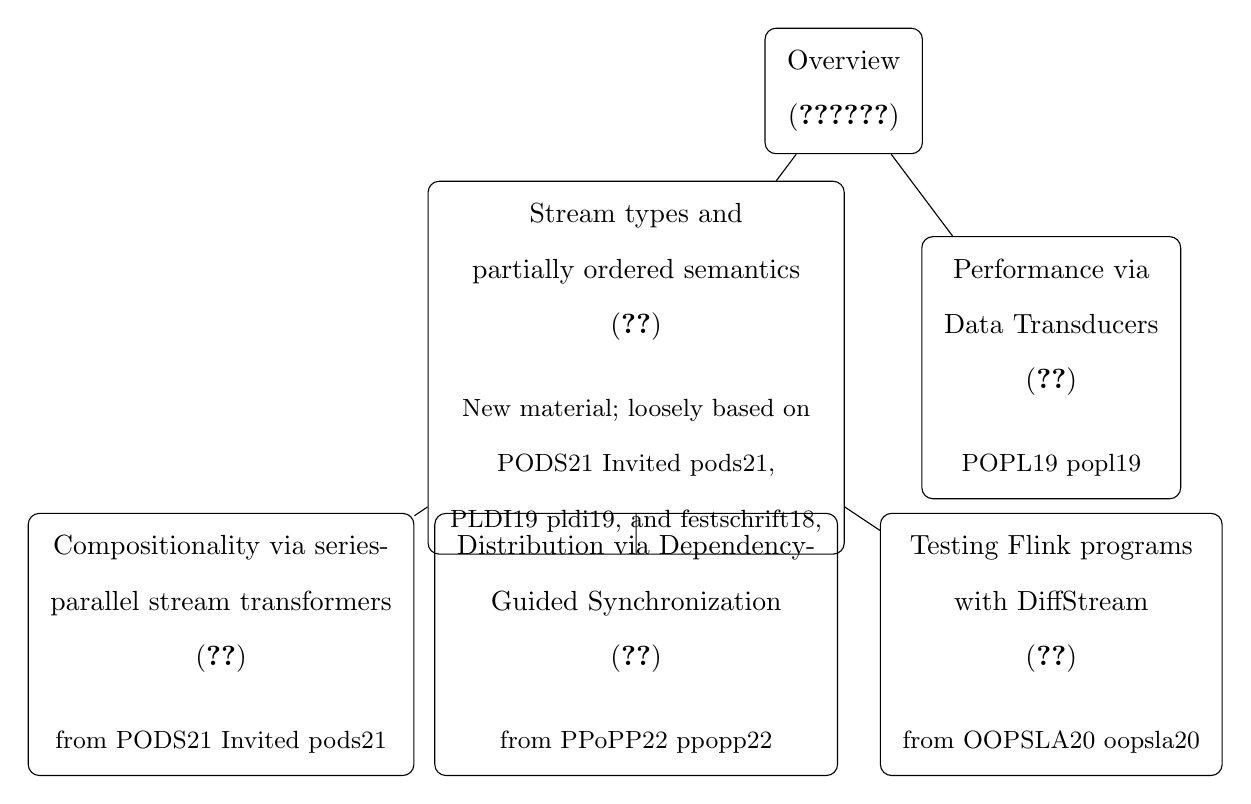
\begin{tikzpicture}[%
    sibling distance=15em,
    level distance=10em,
    every node/.style = {%
      shape=rectangle,
      rounded corners,
      inner sep=0.8em,
      draw,
      align=center
    }
  ]
  \node {
    Overview \\
    (\Cref{cha:intro,cha:background,cha:rw})
  }
    child {
      node {
        Stream types and \\
        partially ordered semantics \\
        (\Cref{cha:foundation}) \\[1em]
        \small New material; loosely based on \\
        \small PODS21 Invited~\citeMain{pods21}, \\
        \small PLDI19~\citeMain{pldi19}, and \citeMain{festschrift18},
      }
      child {
        node {
          Compositionality via series-\\
          parallel stream transformers \\
          (\Cref{cha:composition}) \\[1em]
          \small from PODS21 Invited~\citeMain{pods21}
        }
      }
      child {
        node {
          Distribution via Dependency-\\
          Guided Synchronization \\
          (\Cref{cha:distribution}) \\[1em]
          \small from PPoPP22~\citeMain{ppopp22}
        }
      }
      child {
        node {
          Testing Flink programs \\
          with DiffStream \\
          (\Cref{cha:testing}) \\[1em]
          \small from OOPSLA20~\citeMain{oopsla20}
        }
      }
    }
    child {
      node {
        Performance via \\
        Data Transducers \\
        (\Cref{cha:monitoring}) \\[1em]
        \small POPL19~\citeMain{popl19}
      }
    }
    ;
\end{tikzpicture}

\caption{Overview of the work included in this thesis.}
\label{chapter-overview}
\end{figure}

The structure of the thesis is displayed visually in \Cref{chapter-overview}.
In summary, our contributions are as follows:

\begin{itemize}
\item
We propose a foundational type system for distributed streams based on partially ordered sets.
We show that under our type system, streams can be equivalently viewed as
structured hierarchical data called \emph{batches},
as finite sequences of events called \emph{linearizations},
or as labeled partially ordered sets (traditionally known as pomsets).
In the historical notes, we also discuss how these closely relate to
our earlier synchronization schemas~\citeMain{pods21} and data-trace types~\citeMain{pldi19}.
(\Cref{cha:foundation})

\item
We show how stream operators can be defined compositionally on top of our core type system.~\citeMain{pods21} (\Cref{cha:composition})

\item
We propose \emph{dependency-guided synchronization},
a programming model and system for safe (deterministic and semantics-preserving) distribution~\citeMain{ppopp22}.
(\Cref{cha:distribution})

\item
To detect bugs due to nondeterminism in existing DSPS applications,
we propose \emph{DiffStream}, a differential testing tool~\citeMain{oopsla20}.
In particular, we leverage the partial order viewpoint to specify
ordering requirements, and we test for violations at runtime.
(\Cref{cha:testing})

\item
Towards streaming applications with predictable performance,
we propose \emph{data transducers}, a monitoring formalism and state-machine based intermediate representation~\citeMain{popl19}.
Our formalism is compositional, enabling compilation of high-level
monitoring queries with provable performance bounds.
(\Cref{cha:monitoring})
\end{itemize}

Finally, \Cref{cha:discussion}
contains limitations, unanswered questions, and concluding remarks.

\section{Software}

The work in this thesis is implemented in a number of open-source tools available on GitHub.
\begin{samepage}
\begin{itemize}
\item \githubref{https://github.com/angelhof/flumina}{Flumina} is a parallel programming model for stream processing with safe distribution, written in Erlang with experiments against Flink and Timely Dataflow.
\item \githubref{https://github.com/fniksic/diffstream}{DiffStream} is a differential testing tool for Apache Flink.
\item \githubref{https://github.com/cdstanford/data-transducers}{Data Transducers} is an intermediate representation for streaming with formal performance guarantees, written in Rust.
\end{itemize}
\end{samepage}

\section{Attribution}

Most of the work presented in this thesis was done in close collaboration with my advisor, Rajeev Alur, and other coauthors:
particularly Konstantinos Mamouras (for \Cref{cha:monitoring}) and Konstantinos Kallas and Filip Nikšić (for \Cref{cha:distribution,cha:testing}).
I wrote all the included material in \Cref{cha:intro,cha:background,cha:foundation,cha:composition,cha:discussion}, the material on the programming model in \Cref{cha:distribution}, one of the case studies and other miscellaneous sections in \Cref{cha:testing}, and almost all the material in \Cref{cha:monitoring}.
\Cref{cha:background} incorporates material from my WPE-II written report~\citeMain{wpe2} (of which I am the sole author), and \Cref{cha:rw} integrates some text from all of the papers included in the thesis.

The software repositories Flumina and DiffStream are shared projects with my collaborators, Konstantinos Kallas and Filip Nikšić.
For Flumina, I contributed the experiments and infrastructure with Timely Dataflow in Rust, the Smart Home Power Prediction case study, and documentation.
For DiffStream, I contributed the MapReduce case study and documentation.
The Data Transducers development in Rust is solely my own work.


% \subfile{2-background.tex}
%
% \subfile{3-rw.tex}
%
% \subfile{4-foundation.tex}
%
% \subfile{10-conclusion.tex}

\end{mainf}

%% APPENDICES (OPTIONAL)
% TODO Uncomment if wanted
% \appendix
% APPENDIX START
% \newenvironment{appendixf}{}{}
% \titleformat{\chapter}[hang]{\large\center}{APPENDIX}{0 pt}{} % Old {APPENDIX \thechapter}{0 pt}{ : }
% \titlespacing*{\chapter}{0pt}{-33 pt}{6 pt} % The key value here is the -33 pts, I got to it by old fashioned measuring with a ruler....
%
% \begin{appendixf}
% \addtocontents{toc}{\protect\setcounter{tocdepth}{-1}} % This is to fix how appendices are shown in ToC
% \clearpage
% \chapter{}
% \addtocontents{toc}{\protect\setcounter{tocdepth}{1}} % This is to bring things back to normal
% \addcontentsline{toc}{chapter}{APPENDIX} % You have to write here everything you want the ToC to show including \thechapter if you want numbering
% % \addtocontents{toc}{\protect\setcounter{tocdepth}{-1}} % This is so sections in the appendix are not shown in the ToC
% \subfile{appendix}
% % \addtocontents{toc}{\protect\setcounter{tocdepth}{1}} % This is to bring things back to normal
% \end{appendixf}

% GLOSSARY START
% TODO Uncomment if wanted
% \newenvironment{glossaryf}{}{}
% \titleformat{\chapter}[hang]{\large\center}{GLOSSARY}{0 pt}{} % Old {APPENDIX \thechapter}{0 pt}{ : }
% \titlespacing*{\chapter}{0pt}{-33 pt}{6 pt} % The key value here is the -33 pts, I got to it by old fashioned measuring with a ruler....
%
% \begin{glossaryf}
% \addtocontents{toc}{\protect\setcounter{tocdepth}{-1}} % This is to fix how appendices are shown in ToC
% \clearpage
% \chapter{}
% \addtocontents{toc}{\protect\setcounter{tocdepth}{1}} % This is to bring things back to normal
% \addcontentsline{toc}{chapter}{GLOSSARY} % You have to write here everything you want the ToC to show including \thechapter if you want numbering
% \subfile{glossary}
% \end{glossaryf}


%% BIBLIOGRAPHY
%% Added: separate out primary and other references

\singlespacing
\newenvironment{bibliof}{}{}
\titleformat{\chapter}[hang]{\large\center}{\thechapter}{0 pt}{}
\titlespacing*{\chapter}{0pt}{-25 pt}{6 pt} % The key value here is the -25 pts, I got to it by old fashioned measuring with a ruler....
\begin{bibliof}

% \renewcommand\bibname{BIBLIOGRAPHY}
% \addcontentsline{toc}{chapter}{BIBLIOGRAPHY}
% \bibliographystyle{abbrvnat}
% \bibliography{ref}
% % This is the filename of the bibtex bibliography file (it has to be in the same directory as the main LaTeX file)

\renewcommand\bibname{PRIMARY REFERENCES}
\renewcommand\refname{PRIMARY REFERENCES}
\addcontentsline{toc}{chapter}{PRIMARY REFERENCES}
\bibliographystyleMain{abbrvnat}
\bibliographyMain{ref}
\renewcommand\bibname{BIBLIOGRAPHY}
\renewcommand\refname{BIBLIOGRAPHY}
\addcontentsline{toc}{chapter}{BIBLIOGRAPHY}
\bibliographystyle{abbrvnat}
\bibliography{ref}

\end{bibliof}
%% INDEX (OPTIONAL) - I do not really know how to code this, sorry

\end{document}
